\subsection{Formato del mensaje}
CAN utiliza un formato de mensajes cortos (94 bits) En el mensaje no está explícito ninguna dirección, por este motivo el mensaje puede ser escuchado por todos los nodos de la red \citep{kvaserWEB}.

Los tipos de mensajes son los siguientes:
\begin{itemize}
    \item Frame de datos (Data Frame)
    \item Frame remoto (Remote Framte)
    \item Frame de error (Error Frame)
    \item Frame de sobrecarga (Overload Frame)
\end{itemize}

\subsubsection{Data Frame}
Este es el frame más común. Las partes más importantes son:

\begin{itemize}
\item Campo de arbitraje, el cual determina la prioridad del mensaje
\item El campo de datos, que contiene desde cero hasta ocho bytes de datos
\item El CRC, que está conformado por 15 bits utilizados para calcualr el checksum del mensaje
\item Un campo de ACK. Cualquier controlador que haya recibido el mensaje envía un bit de acuse de recibo al final de cada mensaje. El transmisor comprueba la presencia del bit ACK. En caso de no detectar este bit reenvía el mensaje. Al no poder conocer la dirección de los nodos, no se sabe si el mensaje fue recibido correctamente por el node receptor, solo se sabe que el mensaje fue recibido por uno o más nodos.
\end{itemize}

\subsubsection{Remote Frame}
El frame remoto es un Data Frame con dos diferencias, es marcado como Remote Frame, esto es el bit RTR es recesivo; y por otro lado no hay un campo de datos. Este frame es utilizado para pedir la transmisión de un determinado frame de datos. Por ejemplo si el nodo A transmite un Remote Frame con el campo de arbitraje en 234, entonces el nodo B, reponderá con un frame de datos con el campo de arbitraje seteado a 234 \citep{kvaserWEB}. Este frame es poco utilizado.

\subsubsection{Error Frame}
Este frame se envía cuando un node detecta alguna falla en el mensaje. El envío de este frame provoca la retransmisión inmediata del mensaje. El Error Frame consiste en una bandera, el cual está compuesto por 6 bits del mismo valor, y un Error Delimiter que está compuesto por 8 bits recesivos.

\subsubsection{Overload Frame}
Este frame es similar al frame de error con el mismo formato. Es enviado cuando el nodo está ocupado. Este Frame es muy poco usado. El único controlador que generaba Overload Frame está obsoleto \citep{kvaserWEB}

\subsubsection{CAN estándar y CAN extendido}
El protocolo de comunicación CAN, es un protocolo de multiple acceso con detección de colisión y arbitraje según la prioridad de los mensajes (CSMA/CD+AMP) \citep{texasCAN}. CSMA ya fue estudiado en \ref{subsection:CSMA}. CD+AMP signfica que las colisiones son resueltas mediante arbitración por corrimiento de bits. El identificador con mayor prioridad es el que siempre gana el bus.

El CAN estandar (Figura \ref{fig:StandarCAN}) tiene los siguientes campos:

\begin{figure}[h]
 \centering
 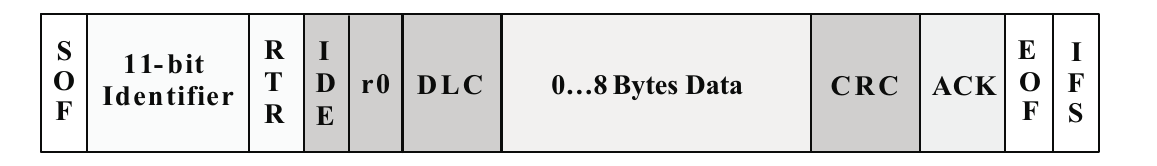
\includegraphics[scale=0.3]{images/Marco_teorico/StandarCAN.png}
  \caption{Frame de mensaje del CAN estándar}
\label{fig:StandarCAN}
\end{figure}

\begin{itemize}
  \item SOF: es el bit dominante de inicio de frame, este marca el comienzo de un mensaje.
  \item Identificador: este es un identificador de 11 bits, en el cual el valor binario más bajo es el de mayor prioridad.
  \item RTR: El bit denominado Remote Transmission Request (RTR) es dominante cuando la información es requerida desde otro nodo. Todos los nodos reciven el pedido, pero el identificador determina node específico.
  \item IDE: Es una extensión del bit identificadorque signfica que se está por transmitir un un identificador estandar CAN sin extensión.
  \item r0: Bit reservado.
  \item DLC: 4 bits que contiene el  número de bytes que van a transmitirse.
  \item Data: Hasta 64 bits, es el mensaje que se transmite.
  \item CRC: Son 16 bits que conforman el Cyclic Redundancy Check (CRC) para chequear la existencia de algún error.
  \item ACK: Todos los nodos que reciben el mensaje correctamente sobreescribe este bit recesivo, indicando que han recibido el mensaje sin errores. Si un nodo detecta un error y detecta la persitencia de este bit recesivo. Con esto, se descarta el mensaje enviado y el nodo transmisor vuelve a enviar el mensaje.
  \item IFS: Son 7 bits que representan el espacio entre frames.Es el tiempo que requiere el controlador para mover el mensaje hasta el buffer de mensajes recibidos.
\end{itemize}

El CAN extendido (Figura \ref{fig:extendedCAN})es idéntico al CAN estándar, salvo por algunos detalles:

\begin{figure}[h]
 \centering
 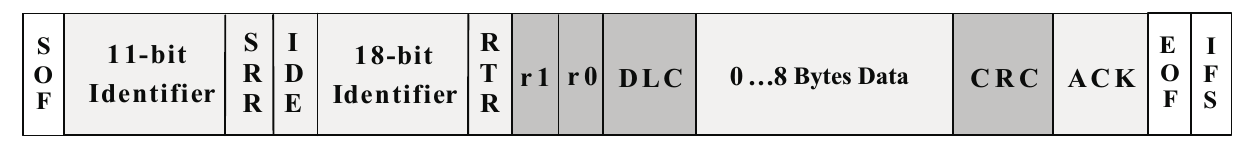
\includegraphics[scale=0.3]{images/Marco_teorico/ExtendedCAN.png}
  \caption{Frame del mensaje del CAN extendido}
\label{fig:extendedCAN}
\end{figure}

\begin{itemize}
  \item SRR: Es el bit de peteción remota subtituta que remplaza al bit RTR del mensaje estándar.
  \item IDE: Un bit recesivo en el identificador de extensión (IDE) indica que siguen más bits de identificación. A este le siguen 18 bits.
  \item r1: Este bit viene después del RTR, es un bit adicional reservado.
\end{itemize}

\subsubsection{Arbitraje}
Cualquier controlador CAN, cuando detecta que el bus está desocupado puede comenzar a transmitir. Esto puede ocacionar que al mismo tiempo, dos o más controladores comiencen a transmitir al mismo tiempo. Este conflicto se resuelve de una manera ingeniosa. El nodo transmisor a medida que transmite los bits, se encuentra monitoreando el bus. Si por ejemplo, el nodo detecta un bit dominante cuando este envío un bit recesivoa, el nodo inmediatamente deja de transmitir y se convierte en un receptor. Cuando el bus se encuentra desocupado, recién vuelve a transmitir \citep{kvaserWEB}.

Una condición importante que se debe cumplir es que dos o más nodos no pueden transmitir el mismo campo de arbitraje.
